\documentclass[a4paper,12pt]{article}
\usepackage{amssymb} % needed for math
\usepackage{amsmath} % needed for math
\usepackage[utf8]{inputenc} % this is needed for german umlauts
\usepackage[ngerman]{babel} % this is needed for german umlauts
\usepackage[T1]{fontenc}    % this is needed for correct output of umlauts in pdf
\usepackage[margin=2.5cm]{geometry} %layout
\usepackage{booktabs}
\usepackage{hyperref}
\hypersetup{pdftitle={Balanced Banana},bookmarks=true,}
\usepackage{graphicx}
\usepackage{csquotes}
\usepackage[nonumberlist]{glossaries}
\usepackage{enumitem}
\usepackage{verbatim}
\usepackage{indentfirst} % Adds indent for the first paragraph after a {/section}


\deftranslation[to=ngerman]{Glossary}{\section{Stichwortverzeichnis}}

\makeatletter
\newenvironment{mycode}
 {\def\@xobeysp{\ }\verbatim\rightskip=0pt plus 6em\relax}
 {\endverbatim}
\makeatother

\setitemize{align=parleft, labelsep=0.5cm}


\makenoidxglossaries

\newglossaryentry{Befehlszeile}
{
	name=Befehlszeile,
	plural={Befehlszeile},
	description={Anwendung, mit der Befehle auf dem Rechner ausgeführt werden.},
}

\newglossaryentry{CPU}
{
	name=CPU,
	plural={CPU},
	description={Central Processing Unit, Kern jedes Rechners um Anwendungen auszuführen},
}

\newglossaryentry{Daemon}
{
	name=Daemon,
	plural={Daemon},
	description={Ein Dienst der Anfragen annimmt und beantwortet.},
}
\newglossaryentry{Client}
{
	name={Client},
	plural={Clients},
	description={Ein Programm auf einem Benutzer PC, welches mit dem Server kommuniziert.}
}

\newglossaryentry{Server}
{
	name={Server},
	plural={Server},
	description={Ein Programm auf einem Server, der die Benutzer (Außenwelt) mit den Arbeitern (Privates Netzwerk) verbindet.}
}

\newglossaryentry{Konfigurationsdatei}
{
	name={Konfigurationsdatei},
	plural={Konfigurationsdateien},
	description={Eine Datei die bestimmte Einstellungen speichert}
}

\newglossaryentry{Benutzer}
{
	name={Benutzer},
	plural={Benutzer},
	description={Eine Person, die dazu in der Lage ist, Befehle auszuführen}
}

\newglossaryentry{Prioritaet}
{
	name={Priorität},
	plural={Prioritäten},
	description={Ein diskretes Maß für Wichtigkeit bzw. Relevanz. Meist eine ganze Zahl, wobei gewisse Werte auch durch vorher definierte Wörter bezeichnet werden können}
}

\newglossaryentry{Arbeiter}
{
	name={Arbeiter},
	plural={Arbeiter},
	description={Ein Programm auf einem Rechner, der Aufgaben ausführt.}
}

\newglossaryentry{Aufgabe}
{
	name={Aufgabe},
	plural={Aufgaben},
	description={Jedes Programm (z.B. Skripte, Simulationen, etc.), das ein Benutzer auf einem Rechenknoten ausführen möchte}
}

\newglossaryentry{Statistik}
{
	name={Statistik},
	plural={Statistiken},
	description={Nützliche Informationen (z.B. Dauer der Task, Statuscode, etc.) über eine Aufgabe, die gesammelt werden sollen.}
}

\newglossaryentry{Web-API}
{
	name={Web-API},
	description={Web-API (Web-Application Programming Interface) ist eine Schnittstelle über das Internet, die eine Sammlung von Funktionen zur Verfügung stellt, die es Benutzern ermöglichen, auf bestimmte Informationen einer Anwendung, eines Betriebssystems oder anderer Dienste zuzugreifen.}
}

\newglossaryentry{Fehlerbehandlung}
{
	name={Fehlerbehandlung},
	plural={Fehlerbehandlungen},
	description={Vorschriften oder Abläufe, die zur Korrektur eines Fehlers dienen.}
}

\newglossaryentry{Parameter}
{
	name={Parameter},
	plural=Parameter,
	description={Eine für die Ausführung eines Programms relevante Variable.}
}

\newglossaryentry{Schnittstelle}
{
	name={Schnittstelle},
	plural=Schnittstellen,
	description={Eine Art Verbindung zwischen zwei oder mehr voneinander unabhängigen Systemen.}
}

\newglossaryentry{Warteschlange}
{
	name=Warteschlange,
	plural=Warteschlangen,
	description={Datenstruktur, in der Aufgaben für die weitere Verwendung zwischengespeichert werden. Kann mit einer Priorität behaftet sein, welche bestimmt, in welcher Reihenfolge die Aufgaben aus der Warteschlange entfernt werden.}
}

\newglossaryentry{Docker-Container}
{
	name=Docker-Container,
	plural=Docker-Container,
	description={Ein Container ist eine Standardeinheit von Software, die Code und alle Abhängigkeiten zusammenfasst, damit die Anwendung auf unterschiedlichen Rechnersystemen läuft.}
}

\newglossaryentry{Docker}
{
	name=Docker,
	plural=Docker,
	description={Ein Programm, mit dessen Hilfe man Aufgaben von dem Host System abkapseln kann.}
}

\newglossaryentry{Docker-Image}
{
	name=Docker-Image,
	plural=Docker-Images,
	description={Ein Bauplan für einen Docker Container.}
}

\newglossaryentry{Datenbank}
{
	name=Datenbank,
	plural=Datenbanken,
	description={Enthalten verschiedene Informationen, so dass Abfragen nach bestimmten Merkmalen effizient möglich sind.}
}

\title{Balanced Banana}
\author{Niklas Lorenz \and Thomas Häuselmann \and Rakan Zeid Al Masri \and Christopher Lukas Homberger \and Jonas Seiler}


%%%%%%%%%%%%%%%%%%%%%%%%%%%%%%%%%%%%%%%%%%%%%%%%%%%%%%%%%%%%%%%%%%%%%%
% Create a shorter version for tables. DO NOT CHANGE               	 %
%%%%%%%%%%%%%%%%%%%%%%%%%%%%%%%%%%%%%%%%%%%%%%%%%%%%%%%%%%%%%%%%%%%%%%
\newcommand\addrow[2]{#1 &#2\\ }

\newcommand\addheading[2]{#1 &#2\\ \hline}
\newcommand\tabularhead{\begin{tabular}{lp{13cm}}
\hline
	}

\newcommand\addmulrow[2]{ \begin{minipage}[t][][t]{2.5cm}#1\end{minipage}%
   &\begin{minipage}[t][][t]{8cm}
    \begin{enumerate} #2   \end{enumerate}
    \end{minipage}\\ }

\newenvironment{usecase}{\tabularhead}
{\hline\end{tabular}}

\usepackage{microtype}

\begin{document}
\pagenumbering{roman}
\begin{titlepage}
    \begin{center}
    
     \vspace*{0.8cm}
 
        
\includegraphics[width=0.5\textwidth]{balancedbanana}
        \vspace*{1cm}
 
        \Huge
        \textbf{Balanced Banana}
 
        \vspace{0.5cm}
        \LARGE
        A Distributed Task Scheduling System
        
        \vspace{0.5 cm}
        \LARGE
        Pflichtenheft
 
        \vspace{1.5cm}

        \large
        \textbf{Niklas Lorenz, Thomas Häuselmann, Rakan Zeid Al Masri, Christopher Lukas Homberger und Jonas Seiler}
 
        \vspace*{0.5cm}

        \textbf{\today}
 
       
        
 
    \end{center}
\end{titlepage}         % Deckblatt.tex laden und einfügen
\setcounter{page}{2}
\tableofcontents          % Inhaltsverzeichnis ausgeben
\clearpage
\pagenumbering{arabic}

\section{Einleitung}
\vspace*{1cm}

Die Verteilung rechenintensiver \glspl{Aufgabe} ist ein in vielen Unternehmen übliches Problem. Wenn ein Team größer wird, so werden auch die verfügbaren Rechenressourcen und die darauf ausgeführten \glspl{Aufgabe} größer und komplexer.\\


Es wird immer schwieriger, die vorhandenen Ressourcen effizient und gerecht an die verschiedenen Mitarbeiter und \glspl{Aufgabe} zu verteilen.
Aktuell stehen individuelle \glspl{Arbeiter} zur Verfügung, die von jedem Mitarbeiter beliebig verwendet werden können. So können \glspl{Aufgabe} nur bearbeitet werden, wenn zum Zeitpunkt der Anfrage ein \gls{Arbeiter} frei steht. Doch das ist weder fair einem einzelnen \gls{Benutzer} gegenüber, noch kann die Hardware dadurch gut ausgelastet werden. Wird eine \gls{Aufgabe} beispielsweise mitten in der Nacht abgeschlossen, ist niemand da, um eine neue \glspl{Aufgabe} ausführen zu lassen. \\


Es gibt auf dem Markt bereits viele Lösungen für dieses Problem, allerdings sind sie sehr komplex und nicht leicht erweiterbar.
Balanced Banana löst dieses Problem maßgeschneidert an die Bedürfnisse des CES. \\

Mit Balanced Banana soll der \gls{Benutzer} sine \gls{Aufgabe} unkompliziert von der \gls{CLI} abschicken können, sodass diese automatisch auf einen bereitstehenden \gls{Arbeiter} verteilt wird. Die \glspl{Aufgabe} sind in \gls{Docker}-Containern von anderen \glspl{Aufgabe} abgetrennt.  \\

Darüber hinaus soll der \gls{Benutzer} durch zusätzliche \glspl{Parameter} in der Lage sein, weitere Einschränkungen und/oder Bedingungen für seine \glspl{Aufgabe} anzugeben.\\

Balanced Banana soll in der Lage sein, die anstehenden \glspl{Aufgabe} effizient auf die verfügbaren \glspl{Arbeiter} zu verteilen. Hierbei werden Größe, \gls{Prioritaet} und gegebenen Einschränkungen berücksichtigt. Um möglichst flexibel einsetzbar zu sein, soll außerdem die \gls{Verteilerlogik} über eine feste \gls{Schnittstelle} jederzeit änderbar sein, sodass Aspekten wie Fairness oder \gls{Turnaround}-Zeit unterschiedliche Relevanz eingeräumt werden kann.

\clearpage
\section{Zielbestimmung}
\subsection{Kundenvorgaben}
\begin{itemize}[nosep]
	
	\item Der \gls{Benutzer} kann seine \gls{Aufgabe} unkompliziert von der \gls{Befehlszeile} abschicken.
	
	\item \gls{Parameter} ermöglichen die Angabe von Einschränkungen und Ansprüchen, wie zum Beispiel \gls{Prioritaet} oder minimal benötigter Arbeitsspeicher.
		
	\item Balanced Banana soll die \glspl{Aufgabe} der \glspl{Benutzer} auf die \glspl{Arbeiter} verteilen.
	
	\item Vom \gls{Benutzer} in Auftrag gegebene \glspl{Aufgabe} sollen automatisch gestartet werden.
	
	\item Balanced Banana sammelt \glspl{Statistik} über \glspl{Aufgabe}. Die \glspl{Statistik} sind von dem \gls{Auftraggeber} einsehbar.
	
	\item Öffentliche \glspl{Statistik} sollen über eine \gls{Web-API} mit \glspl{HTTP-Anfrage} bereitgestellt werden.
	
	\item Die Anzahl der \glspl{Arbeiter} ist variabel.
	
	\item Der \gls{Benutzer} kann eine \gls{Prioritaet} für jede \gls{Aufgabe} angeben.
	
	\item Der \gls{Benutzer} soll benachrichtigt werden, sobald eine von ihm in Auftrag gegebene \gls{Aufgabe} erledigt ist oder fehlschlägt.
	
	\item Balanced Banana verfügt über eine ausführliche Dokumentation und Bedienungsanleitung.

\end{itemize}

\subsection{Eigene Ergänzungen}
\begin{itemize}[nosep]

	\item Der \gls{Benutzer} kann eine von ihm in Auftrag gegebene \gls{Aufgabe} pausieren.	
	
	\item Balanced Banana kann die verbleibende Restlaufzeit für die nicht beendeten \glspl{Aufgabe} vorhersagen.
	
	\item Die Rückmeldung nach Beendigung einer \gls{Aufgabe} kann in verschiedenen Sprachen erfolgen.
	
	\item \gls{Benutzer} können den Status von \glspl{Aufgabe}, die nicht von ihnen in Auftrag gegeben wurden, einsehen und 	sich über Änderungen benachrichtigen lassen.
	
	\item Der \gls{Benutzer} kann einen verzögerten Start einer \gls{Aufgabe} anfordern.
	
\end{itemize}

\subsection{Abgrenzungskriterien}
\begin{itemize}[nosep]

	\item Balanced Banana führt die in Auftrag gegebenen \glspl{Aufgabe} nicht persönlich aus, sondern übergibt die \gls{Aufgabe} an einen \gls{Arbeiter}.
	
	\item Balanced Banana ignoriert die Ausgabe der \glspl{Aufgabe}. Balanced Banana ist ausschließlich für die Verteilung der \glspl{Aufgabe} verantwortlich.

	\item Balanced Banana ignoriert Fehler der \glspl{Aufgabe}. Eine \gls{Fehlerbehandlung} soll von den \glspl{Aufgabe} oder dem \gls{Auftraggeber} erfolgen.

	\item Die erhobenen \glspl{Statistik} werden nicht ausgewertet. Die \glspl{Statistik} werden zur Weiterverwendung durch die \glspl{Benutzer} erhoben.
	
	\item Balanced Banana garantiert nicht, dass getrennte \glspl{Aufgabe} miteinander kommunizieren können.
	
\end{itemize}

\clearpage
\section{Szenarien}

\subsection{Einreihen einer \gls{Aufgabe} in \gls{Warteschlange}}
Tom möchte eine Katzensimulation simulieren lassen.
Tom startet auf seinem PC den BalancedBanana-\gls{Client}. Dieser verbindet sich im Hintergrund mit dem \gls{Server} und authentifiziert Tom.
Nun reiht Tom seine Simulation auf der \gls{Befehlszeile} mit normaler \gls{Prioritaet} ein.
Tom sieht, dass alle \glspl{Arbeiter} ausgelastet sind und dass er an zweiter Stelle in  der \gls{Warteschlange} steht.
Nach zwei Stunden sieht Tom erneut nach und stellt fest, dass er nun an vorderer Stelle in der \gls{Warteschlange} steht.
Nach drei weiteren Stunden sieht er, dass seine \gls{Aufgabe} aus der \gls{Warteschlange} verschwunden ist und er eine E-Mail erhalten hat.
In dieser steht, dass seine \gls{Aufgabe} in 43 Minuten abgeschlossen wurde er erhält einen Link mit dem er die Ausgabe seiner \gls{Aufgabe} einsehen kann.

\subsection{Aufwerten der \gls{Prioritaet}}
Peter möchte eine wichtige Bauteilsimulation rechnen lassen.
Dazu startet Peter den BalancedBanana-\gls{Client} und reiht seine \gls{Aufgabe} mit normaler \gls{Prioritaet} ein.
Nachdem Peter nach 3 Stunden keine Rückmeldung bekommen hat, prüft er die \gls{Warteschlange} und sieht das Tom ein Duzent Katzensimulationen mit hoher \gls{Prioritaet} eingereiht hat.
Genervt beendet Peter seinen PC und hofft das seine Simulation bis morgen abgeschlossen ist.
Am nächsten morgen bemerkt Peter das Tom ein weiteres Duzent Katzensimulationen mit erneut hoher \gls{Prioritaet} eingereiht hat.
24 Stunden nach Einreihung seiner \gls{Aufgabe} wird nun die \gls{Prioritaet} dieser automatisch erhöht und hat nun ebenfalls hohe \gls{Prioritaet}.
Peter bemerkt das seine \gls{Aufgabe} nun in der \gls{Warteschlange} langsam nach vorne rückt und schließlich gestartet wird. 
Nach einiger Zeit erhält Peter eine E-Mail mit dem Ergebnis seiner Simulation.

\section{Systemmodelle}

\includegraphics[width=\textwidth]{Anwendungsmöglichkeiten}
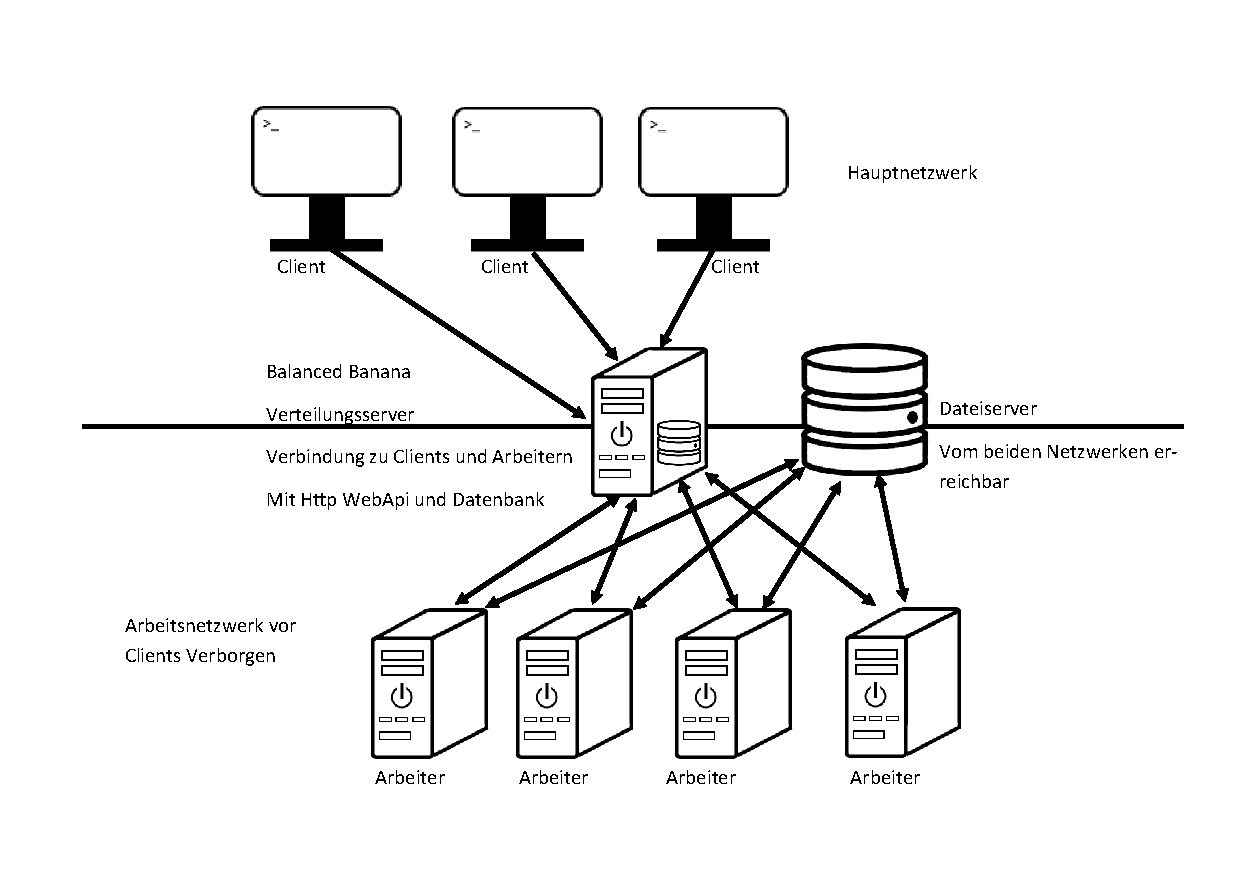
\includegraphics[width=\textwidth]{Systemmodelle/Systemaufbau}

Den Kern des Systems stellt der \gls{Server} dar. Er ist in der Lage über ein von Nutzern benutzbares Netzwerk Anfragen von den einzelnen \glspl{Client} entgegenzunehmen und sie zu verwalten.
Außerdem enthält er eine \gls{Datenbank}, in der sämtliche \glspl{Statistik} gespeichert werden, sowie einen HTTP Dienst, der Anfragen auf \gls{Statistik} beantwortet und einen SMTP-Dienst, der die \glspl{Benutzer} benachrichtigt. An einer weiteren Schnittstelle ist er an ein von Außen nicht sichtbares Netzwerk angeschlossen, in dem sich die einzelnen \glspl{Arbeiter} befinden. Der \gls{Server} kann Anfragen direkt an die sie in diesem Netz verteilen, ohne dass die \gls{Arbeiter} von außerhalb des versteckten Netzes gesehen werden können. Außerdem gibt es ein geteiltes Netzwerk-Dateisystem, das von allen Rechnern in beiden Netzwerken, dem öffentlichen Netz und dem versteckten Arbeiternetz, erreichbar ist. Hier können Daten und Programme gespeichert werden, die für die erstellten \glspl{Aufgabe} benötigt werden.

\subsection{Ablaufdiagramme}
\subsubsection{Systeminitialisierung}
Dieses Ablaufdiagramm soll grob den Ablauf der Systeminitialisierung skizzieren, bei der aus einzelnen Rechnern das ganze System gebaut wird.\\

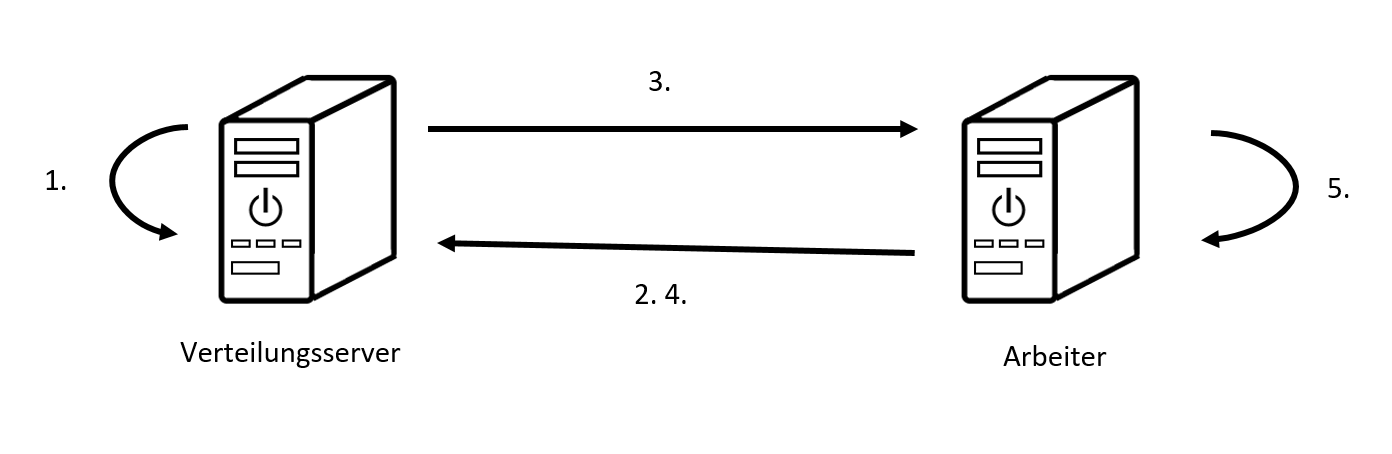
\includegraphics[width=\linewidth]{Systemmodelle/Models/Init.PNG}
\\
1. Der \gls{Server} fängt an, auf Anfragen von Nutzern und Arbeitern zu hören. Falls die \gls{Warteschlange} beim letzten System Stopp nicht leer war, lädt er außerdem alle noch nicht bearbeiteten \glspl{Aufgabe} in seine \gls{Warteschlange}.\\
2. Ein \gls{Arbeiter} schickt eine Anfrage an alle Rechner im Netzwerk, ob es sich bei ihnen um einen \gls{Server} handelt. \\
3. Der \gls{Server} bestätigt dem \gls{Arbeiter}, dass er ein \gls{Server} ist.\\
4. Der \gls{Arbeiter} teilt dem \gls{Server} mit, dass er bereitsteht um bei jenem eingereichte \glspl{Aufgabe} zu bearbeiten.\\
5. Der \gls{Arbeiter} wartet auf \glspl{Aufgabe} vom \gls{Server}.

\subsubsection{Systemabbau}
Im Folgenden soll der Ablauf zur Außerbetriebnahme des Systems für beispielsweise Wartungsarbeiten skizziert werden.\\

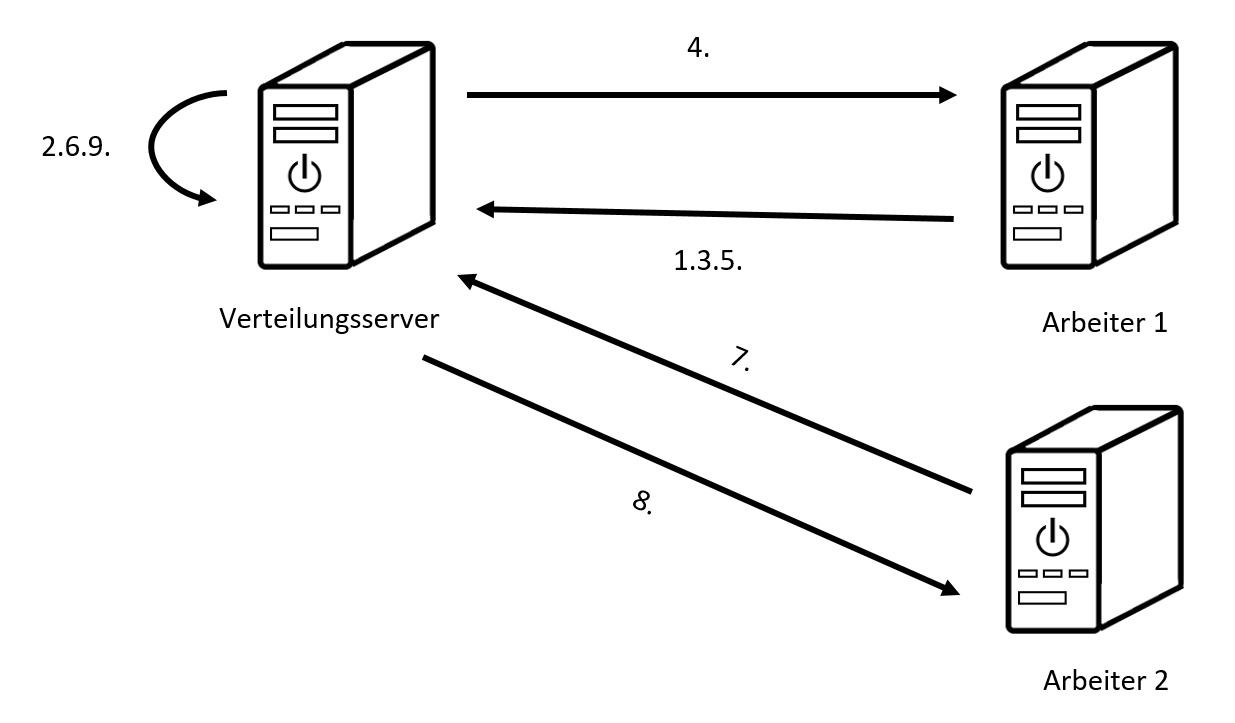
\includegraphics[width=\linewidth]{Systemmodelle/Models/Shutdown.PNG}
\\
Manuelle Abmeldung eines einzelnen \gls{Arbeiter}s:\\
1. Der \gls{Arbeiter}1 soll vom System abgemeldet werden und meldet sich deshalb beim \gls{Server} ab, rechnet aber seine aktuelle \gls{Aufgabe} noch zu ende.\\
2. Der \gls{Server} plant den \gls{Arbeiter}1 aus.\\
3. Der \gls{Arbeiter}1 meldet den Abschluss der \gls{Aufgabe}.\\
4. Der \gls{Server} benachrichtigt den \gls{Arbeiter}1, dass er befreit ist.\\
5. Der \gls{Arbeiter}1 bestätigt dem \gls{Server}, dass er die Befreiung erhalten hat.\\
Herunterfahren des gesamten Systems:\\
6. Der \gls{Server} wartet, bis alle \gls{Arbeiter} mit ihren aktuellen \glspl{Aufgabe} fertig sind, gibt sie dann frei (siehe 4. bis 5.) und speichert schon mal alle sich noch in der \gls{Warteschlange} befindenden \glspl{Aufgabe} ab.\\
7. Der letzte \gls{Arbeiter} (\gls{Arbeiter}2) meldet den Abschluss seiner \gls{Aufgabe}.
8. Der \gls{Server} verarbeitet diese Meldung normal und gibt auch ihn frei.
9. Der \gls{Server} beendet seinen Dienst.

\subsection{Aufgabenverarbeitung}
Dieses Diagramm beschreibt den groben Verlauf der Bearbeitung einer \gls{Aufgabe} von der Erstellung bis zur Benachrichtigung beim Abschluss.\\
%Hier Bild einfügen
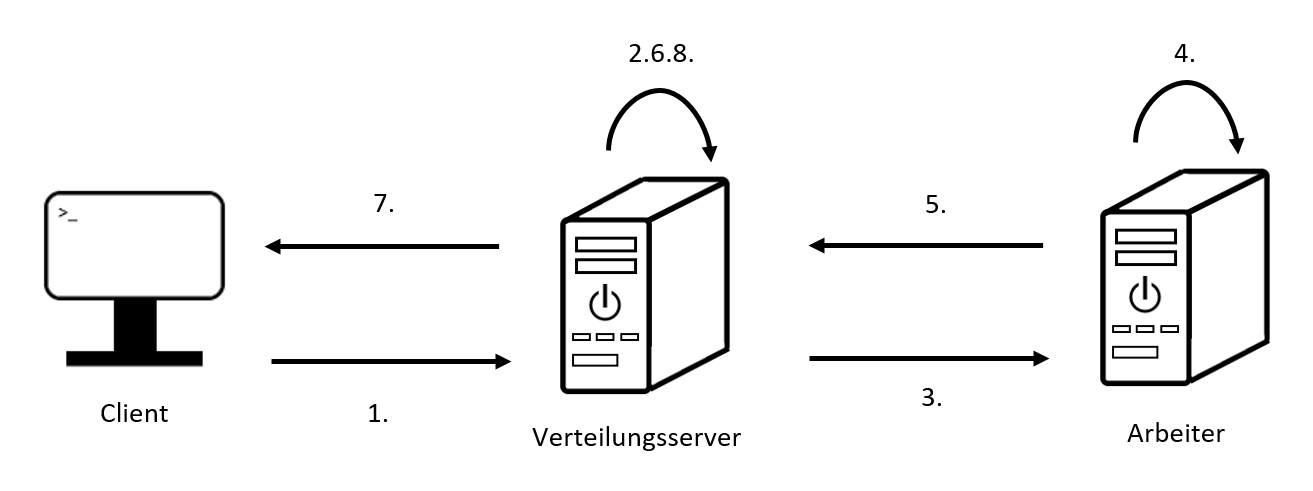
\includegraphics[width=\linewidth]{Systemmodelle/Models/Scheduling.PNG}
\\
1. Der \gls{Benutzer} erstellt eine \gls{Aufgabe} und sendet sie an den \gls{Server}.
2. Der \gls{Server} plant die \gls{Aufgabe} ein und wartet, bis ein \gls{Arbeiter} genug Ressourcen zur Verfügung stellt, damit die \gls{Aufgabe} bearbeitet werden kann.\\
3. Der \gls{Server} sendet die \gls{Aufgabe} an den \gls{Arbeiter}.\\
4. Der \gls{Arbeiter} bearbeitet die \gls{Aufgabe}.\\
5. Der \gls{Arbeiter} meldet den Abschluss der \gls{Aufgabe} beim \gls{Server}.\\
6. Der \gls{Server} speichert \glspl{Statistik} über die \gls{Aufgabe} in der \gls{Datenbank} ab.\\
7. Der \gls{Server} meldet den Abschluss der \gls{Aufgabe} an den \gls{Benutzer}, sofern er noch im System angemeldet ist und auf eine Antwort wartet.\\
8. Der \gls{Server} verschickt eine E-Mail an die bei der Erstellung der \gls{Aufgabe} spezifizierte Adresse, die den \gls{Benutzer} auf den Abschluss seiner \gls{Aufgabe} hinweist.

\subsubsection{Notfall Aufgabenverarbeitung}
Dieses Diagramm veranschaulicht den Verlauf einer Notfall Verteilung. Eine Notfall Verteilung bezeichnet eine \gls{Aufgabe}, die schnellstmöglich bearbeitet werden muss.\\
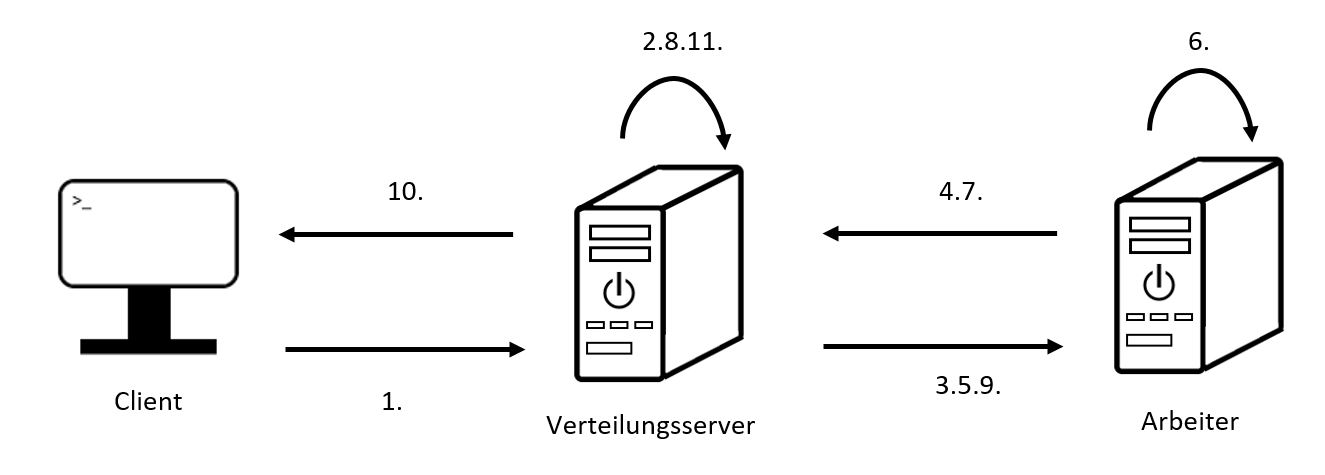
\includegraphics[width=\linewidth]{Systemmodelle/Models/Emergency-Scheduling.PNG}
\\
1. Der \gls{Client} sendet eine Notfall-Anfrage an den \gls{Server}.\\
2. Der \gls{Server} sucht sich einen geeigneten \gls{Arbeiter}.\\
3. Der \gls{Server} weist den \gls{Arbeiter} dazu an, seine Arbeit zu unterbrechen.\\
4. Der \gls{Arbeiter} meldet, dass er seine Arbeit unterbrochen hat.\\
5. Der \gls{Server} übermittelt die Notfall \gls{Aufgabe} an den \gls{Arbeiter}.\\
6. Der \gls{Arbeiter} bearbeitet die Notfall \gls{Aufgabe}.\\
7. Der \gls{Arbeiter} benachrichtigt den \gls{Server} über den Abschluss des Notfalls.\\
8. Der \gls{Server} speichert \glspl{Statistik} und Ergebnis der Notfall \gls{Aufgabe}.\\
9. Der \gls{Server} weist den \gls{Arbeiter} an, seine unterbrochene Arbeit fortzusetzen.\\
10. Der \gls{Server} benachrichtigt den \gls{Client} über den Abschluss des Notfalls.\\
11. Der \gls{Server} löst das Versenden der Benachrichtigungs E-Mail aus.

\clearpage

\section{Produkteinsatz}
\begin{itemize}
\begin{minipage}[t]{\linewidth}
\item \textbf{Zielgruppe}\newline
Balanced Banana ist für die Verwendung durch die Mitarbeiter am Chair for Embedded Systems (CES) des Karlsruher Institut für Technologie (KIT) gedacht.\newline
Den Mitarbeitern soll die Benutzung der \gls{Arbeiter} erleichtert werden, indem die Verteilung der \glspl{Aufgabe} automatisch erfolgt. Somit soll garantiert werden, dass die \glspl{Aufgabe} sich gegenseitig möglichst wenig stören.\newline
Durch die Vermeidung von Situationen, in denen mehrere Personen \glspl{Aufgabe} auf dem selben \gls{Arbeiter} ausführen, während einer oder mehrere andere \glspl{Arbeiter} unbeschäftigt sind, soll die Leistungsfähigkeit sowie allgemeine Zufriedenheit und Harmonie gesteigert werden.
\end{minipage}
\\

\begin{minipage}[t]{\linewidth}
\item \textbf{Verwendungszweck}\newline
Balanced Banana dient dazu, Simulationen und andere rechenintensive \glspl{Aufgabe} auf eigens zu diesem Zweck gedachte Rechner (\gls{Arbeiter}) zu verteilen.\newline
Oftmals fallen \glspl{Aufgabe} an, die von einem Computer berechnet werden können und sollen. Nicht immer ist der eigene Rechner jedoch dieser \gls{Aufgabe} gewachsen. Damit sich \gls{Benutzer} und \gls{Aufgabe} also nicht um Rechenzeit streiten, werden die anstehenden \glspl{Aufgabe} auf einen Pool von Arbeitern verteilt, die speziell für diesen Zweck zur Verfügung stehen. Das Verteilen wird von Balanced Banana übernommen.
\end{minipage}
\\

\begin{minipage}[t]{\linewidth}
\item \textbf{Produktaufbau}\newline
Balanced Banana ist den Aufgabengebieten entsprechend in drei Teile aufgeteilt:\newline
1. Der \gls{Client} (\gls{Benutzer}): Verantwortlich für die Interaktion des Benutzers mit dem Produkt auf der \gls{Befehlszeile}.\newline
2. Der \gls{Scheduler} (\gls{Server}): Verantwortlich für das effiziente Verteilen der \glspl{Aufgabe} auf dem Arbeiterpool. Agiert als Mittelmann zwischen \gls{Benutzer} und \gls{Arbeiter}.\newline
3. Der \gls{Arbeiter} (Worker): Verantwortlich für Ausführung, Pausieren und Abbruch der \glspl{Aufgabe} auf den Arbeitern (spezielle Rechner für die Aufgabenverarbeitung).
\end{minipage}
\end{itemize}
\newpage

\newpage

\section{Funktionale Anforderungen}

\subsection{Übersicht der  Funktionalen Anforderungen}

\begin{itemize}[nosep]
\leftskip=0.5cm

\item[FA1]	\gls{Client} verbindet sich beim Starten mit dem Server.
\item[FA2] Benutzer authentifiziert sich über den \gls{Client} gegenüber dem Server.
\item[FA3] Benutzer kann eine Aufgabe über den \gls{Client} einreihen.
\item[FA4] Benutzer kann Parameter übergeben.
\item[FA41]	\gls{Client} speichert voreingestellte Parameter in \gls{Configfile}.
\item[FA42]	Benutzer kann Parameter über \gls{Configfile} übergeben.
\item[FA43] Benutzer kann \gls{Prioritaet} einer Aufgabe festlegen.
\item[FA44] Benutzer kann minimale und maximale Anzahl genutzer Kerne festlegen.
\item[FA45] Benutzer kann maximal nutzbaren Arbeitsspeicher festlegen.
\item[FA46] Benutzer kann das benutzte Betriebssystem festlegen.
\item[FA47] Benutzer kann angeben, ob der \gls{Client} blockieren soll, bis die Aufgabe beendet ist.
\item[FA48] Benutzer übergibt Pfad zu der Aufgabe.
\item[FA49] Falls der Benutzer keine Parameter übergibt, werden Standardwerte benutzt.
\item[FA5] Benutzer kann den Status einer Aufgabe einsehen.
\item[FA6] Benutzer bekommt Benachrichtigung über abgeschlossene Aufgabe.
\item[FA7] Server erstellt regelmäßige Sicherungen von laufenden Aufgaben.
\item[FA8] Benutzer kann die Ausgabe seiner Aufgabe anfordern.
\item[FA9] \gls{Benutzer} kann erhobene \glspl{Statistik} abfragen.
\end{itemize}
\newpage

\subsection{Erläuterung der funktionalen Anforderungen}

\begin{itemize}[nosep]
	\leftskip=0.5cm
	\begin{minipage}[t]{\linewidth}
		\item[FA1] \textbf{\gls{Client} verbindet sich beim Starten mit dem Server.}
		\subitem \textbf{Erklärung:} Beim Starten des \gls{Client} soll dieser sich automatisch mit dem \gls{Server} verbinden.
		\subitem \textbf{Voraussetzung(en):} Keine.
		\subitem \textbf{Nachbedingung(en):}
		\subsubitem \textbf{Erfolg:} Der \gls{Client} hat sich mit dem \gls{Server} verbunden.
		\subsubitem \textbf{Misserfolg:} Der \gls{Client} konnte sich nicht mit dem \gls{Server} verbinden. Eine entsprechende Fehlermeldung wird ausgegeben.
	\end{minipage}
	\newline
	\\
	
	\begin{minipage}[t]{\linewidth}
		\item[FA2] \textbf{Benutzer authentifiziert sich über den \gls{Client} gegenüber dem Server.}
		\subitem \textbf{Erklärung:} Bevor der Benutzer Befehle ausführen kann, muss dieser sich authentifziert haben.
		\subitem \textbf{Voraussetzung(en):} Der Client hat sich mit dem Server verbunden.
		\subitem \textbf{Nachbedingung(en):} 
		\subsubitem \textbf{Erfolg:} Der \gls{Benutzer} wurde authentifiziert.
		\subsubitem \textbf{Misserfolg:} Der \gls{Benutzer} konnte nicht authentifiziert werden. Eine entsprechende Fehlermeldung wird ausgegeben.
		\subitem \textbf{Details:} Bevor der Benutzer eine Aufgabe einreihen kann (FA3) oder den Status seiner Aufgaben einsehen kann (FA6), muss sich dieser authentifizieren. Dies führt der Client automatisch durch. Falls notwendig, wird der \gls{Benutzer} aufgefordert ein Passwort einzugeben.
	\end{minipage}
    \newline
    \\
    
    \begin{minipage}[t] {\linewidth}
    	\item[FA3] \textbf{Benutzer kann eine Aufgabe über den \gls{Client} einreihen.}
    	\subitem \textbf{Erklärung:} Benutzer kann eine Aufgabe mit Parametern zur Bearbeitung einreihen.
    	\subitem \textbf{Voraussetzung(en):} Der \gls{Benutzer} hat sich gegenüber dem \gls{Server} authentifiziert.
    	\subitem \textbf{Nachbedingung(en):}
    	\subsubitem \textbf{Erfolg:} Die Aufgabe wird in eine Warteschlange eingereiht. Der \gls{Benutzer} bekommt eine Rückmeldung mit der Aufgaben ID.
    	\subsubitem \textbf{Misserfolg:} Die Aufgabe wird nicht eingereiht. Der Benutzer bekommt eine entsprechende Fehlermeldung.
    	\subitem \textbf{Details:} Der \gls{Benutzer} kann über die \gls{Befehlszeile} eine Aufgabe einreihen. Dabei kann er Parameter mit übergeben (FA4). Falls der Benutzer keine Parameter mit übergibt werden Standardparameter verwendet (FA49).
   \end{minipage}
   \newline
   \\
	
	%\item[FA30] Benutzer kann Parameter übergeben %evtl auf FA20 verweisen
	\begin{minipage}[t]{\linewidth}
		\item[FA4] \textbf{Benutzer kann Parameter übergeben.}
		\subitem \textbf{Erklärung:} Bei der Einreihung einer Aufgabe, können weiter Parameter übergeben werden.
		\subitem \textbf{Voraussetzung(en):}Eine Aufgabe soll eingereiht werden.
		\subitem \textbf{Nachbedingung(en):}
		\subsubitem \textbf{Erfolg:} Der Befehl wird mit den angegebenen Parametern eingereiht.
		\subsubitem \textbf{Misserfolg:} Die Aufgabe wird nicht eingereiht. Eine entsprechende Fehlermeldung wird ausgegeben.
		\subitem \textbf{Details:} Wenn eine Aufgabe eingereiht wird, kann der \gls{Benutzer} noch weitere Parameter hinzufügen. Diese können in einer \gls{Configfile} übergeben werden (FA42). Falls keine Parameter eingegeben wurden, werden Standardparameter verwendet (FA49).
		Können mehrere Rechner für eine Aufgabe verwendet werden, so wird zuerst nach minimalem Arbeitsspeicher und danach nach minimalen Kernen ausgesucht.
	\end{minipage}
	\pagebreak
	
	\begin{minipage}[t]{\linewidth}
		\item[FA41] \textbf{\gls{Client} speichert voreingestellte Parameter in \gls{Configfile}.}
		\subitem \textbf{Erklärung:} Standardparameter werden einer \gls{Configfile} gespeichert.
		Diese können bearbeitet werden. Zur einfachen Einreihung können alle Parameter durch eine \gls{Configfile} angegeben werden.
		\subitem \textbf{Vorraussetzungen:} Keine.
		
	\end{minipage}
	\newline
	\\
	
	\begin{minipage}[t]{\linewidth}
		\item[FA42] \textbf{Benutzer kann Parameter über \gls{Configfile} übergeben.}
		\subitem \textbf{Erklärung:} Gibt der Benutzer Parameter bei der Einreihung einer Aufgabe nicht ein, so werden diese von der \gls{Configfile} bezogen.
		\subitem \textbf{Vorraussetzungen:} Eine Aufgabe soll eingereiht werden.
		\subitem \textbf{Nachbedingung:}
		\subsubitem \textbf{Erfolg:} Fehlende Parameter wurden aus der \gls{Configfile} bezogen.
		\subsubitem \textbf{Misserfolg:} Fehlende Parameter werden auf Standardwerte gesetzt.
		\subitem \textbf{Details:} Werden Parameter bei der Einreihung einer Aufgabe nicht weiter spezifiziert, so werden diese aus der \gls{Configfile} gelesen. Sind diese dort ebenfalls nicht spezifiziert, so werden diese auf Standardwerte gesetzt.
	\end{minipage}
	\newline
	\\
	
	\begin{minipage}[t]{\linewidth}
		\item[FA43] \textbf{Benutzer kann \gls{Prioritaet} einer Aufgabe festlegen.}
		\subitem \textbf{Erklärung:} \gls{Benutzer} kann seine Aufgabe mit einer \gls{Prioritaet} versehen.
		\subitem \textbf{Voraussetzung(en):} Eine Aufgabe soll eingereiht werden.
		\subitem \textbf{Nachbedingung(en):}
		\subsubitem \textbf{Erfolg:} Die Aufgabe wird mit der gewünschten \gls{Prioritaet} in die Warteschlange eingereiht.
		\subsubitem \textbf{Misserfolg:} Die Aufgabe wird nicht eingereiht. Eine entsprechende Fehlermeldung wird ausgegeben.
		\subitem \textbf{Details:} Ein \gls{Benutzer} kann einer eingereihten Aufgabe eine \gls{Prioritaet} geben. Diese bestimmt welche Position die Aufgabe in der Warteschlange bekommt. Es gibt vier \glspl{Prioritaet}: Low, Normal, High, Emergency (von niedrig bis hoch sortiert). Eine höhere \gls{Prioritaet} bewirkt ein Einreihen weiter vorne in der Warteschlange. Bei zwei Aufgaben mit gleicher Priorität entscheidet der Zeitpunkt der Einreihung.
    \end{minipage}	
	\newline
	\\
	
	\begin{minipage}[t]{\linewidth}
		\item[FA44] \textbf{Benutzer kann minimale und maximale Anzahl genutzer Kerne festlegen.}
		\subitem \textbf{Erklärung:} \gls{Benutzer} kann eine minimale und maximale Anzahl nutzbarer Kerne als Parameter angeben.
		\subitem \textbf{Voraussetzung(en):} Eine Aufgabe soll eingereiht werden.
		\subitem \textbf{Nachbedingung(en):}
		\subsubitem \textbf{Erfolg:} Die Aufgabe wird mit der gewünschten minimalen und maximalen Anzahl Kerne als Parameter in die Warteschlange eingereiht.
		\subsubitem \textbf{Misserfolg:} Die Aufgabe wird nicht eingereiht. Eine entsprechende Fehlermeldung wird ausgegeben.
		\subitem \textbf{Details:} Ein \gls{Benutzer} kann einer eingereihten Aufgabe eine minimale und maximale Anzahl nutzbarer Kerne zuweisen. Die Aufgabe wird dann mindestens die spezifizierte Angabe Kerne nutzen können und maximal die spezifizierte Anzahl Kerne nutzen können.
	\end{minipage}
	\newline
	\\
	
	\begin{minipage}[t]{\linewidth}
		\item[FA45] \textbf{Benutzer kann minimal und maximal nutzbaren RAM festlegen.}
		\subitem \textbf{Erklärung:} Erlaubt es dem \gls{Benutzer} eine minimale bzw. maximale Menge Arbeitsspeicher als Parameter anzugeben.
		\subitem \textbf{Voraussetzung(en):} Eine Aufgabe soll eingereiht werden.
		\subitem \textbf{Nachbedingung(en):}
		\subsubitem \textbf{Erfolg:} Die Aufgabe wird mit der gewünschten minimalen und maximalen Größe des nutzbaren Arbeitsspeichers als Parameter in die Warteschlange eingereiht.
		\subsubitem \textbf{Misserfolg:} Die Aufgabe wird nicht eingereiht. Eine entsprechende Fehlermeldung wird ausgegeben.
		\subitem \textbf{Details:} Ein \gls{Benutzer} kann einer eingereihten Aufgabe eine minimale und maximale Größe nutzbaren RAMs zuweisen. Die Aufgabe wird dann mindestens die minimale Größe und höchstens die maximale Größe nutzen können.
	\end{minipage}
	\newline
	\\
	
	\begin{minipage}[t]{\linewidth}
		\item[FA46] \textbf{Benutzer kann das benutzte Betriebssystem festlegen.}
		\subitem \textbf{Erklärung:} Erlaubt es dem \gls{Benutzer} das Betriebssystem, auf dem die Aufgabe ausgeführt werden soll, als Parameter auszuwählen.
		\subitem \textbf{Voraussetzung(en):} Eine Aufgabe soll eingereiht werden.
		\subitem \textbf{Nachbedingung(en):}
		\subsubitem \textbf{Erfolg:} Die Aufgabe wird mit dem gewünschten Betriebssystem als Parameter eingereiht.
		\subsubitem \textbf{Misserfolg:} Die Aufgabe wird nicht eingereiht. Eine entsprechende Fehlermeldung wird ausgegeben.
		\subitem \textbf{Details:} Ein \gls{Benutzer} kann einer eingereihten Aufgabe ein gewünschtes Betriebssystem als Parameter zuweisen. Die Aufgabe wird dann auf dem gewünschten Betriebssystem ausgeführt.
	\end{minipage}
	\newline
	\\
	
	\begin{minipage}[t]{\linewidth}
		\item[FA47] \textbf{Benutzer kann angeben, ob der \gls{Client} blockieren soll, bis die Aufgabe beendet ist.}
		\subitem \textbf{Erklärung:} Erlaubt es dem \gls{Benutzer} anzugeben, ob der Client keine weiteren Befehle annehmen soll, bis die einreihende Aufgabe beendet ist.
		\subitem \textbf{Voraussetzung(en):} Eine Aufgabe soll eingereiht werden.
		\subitem \textbf{Nachbedingung(en):}
		\subsubitem \textbf{Erfolg:} Die Aufgabe wird eingereiht. Der Benutzer kann keine weiteren Befehle über den Client eingeben, bis die eingereihte Aufgabe beendet ist.
		\subsubitem \textbf{Misserfolg:} Die Aufgabe wird nicht eingereiht. Eine entsprechende Fehlermeldung wird ausgegeben.
		\subitem \textbf{Details:} Ein \gls{Benutzer} kann zu einer eingereihten Aufgabe spezifizieren, ob der Client Eingaben blockieren soll, bis die eingereihte Aufgabe beendet wurde. Dies ist nützlich für Skripte für z.B Aufgaben, die abhängig von dem Ergebnis von anderen Aufgaben sind.
	\end{minipage}
	\newline
	\\
	
	\begin{minipage}[t]{\linewidth}
		\item[FA48] \textbf{\gls{Benutzer} übergibt Pfad zu der Aufgabe.}
		\subitem \textbf{Erklärung:} Der \gls{Benutzer} ist aufgefordert einen Dateipfad als Parameter an eine Einreihung anzuhängen, der zu der Aufgabe zeigt.
		\subitem \textbf{Voraussetzung(en):} Eine Aufgabe soll eingereiht werden.
		\subitem \textbf{Nachbedingung(en):}
		\subsubitem \textbf{Erfolg:} Die angegebene Aufgabe wird eingereiht.
		\subsubitem \textbf{Misserfolg:} Die Aufgabe wird nicht eingereiht. Eine entsprechende Fehlermeldung wird ausgegeben.
		\subitem \textbf{Details:} Ein \gls{Benutzer} wird aufgefordert einen Dateipfad als Parameter an einen Einreihungsbefehl anzuhängen. Hierfür existiert kein Standardparameter. Die Ausführbarkeit der Aufgabe wird bis zum Aufgabenstart nicht überprüft.
	\end{minipage}
	\newline
	\\
	
	\begin{minipage}[t]{\linewidth}
		\item[FA49] \textbf{Falls der \gls{Benutzer} keine Parameter übergibt, werden Standardwerte benutzt.}
		\subitem \textbf{Erklärung:} Sollte der \gls{Benutzer} keine Parameter über die Befehlszeile übergeben oder nicht in einer Configfile spezifiziert haben, werden für bestimmte Parameter Standardwerte ausgewählt
		\subitem \textbf{Voraussetzung(en):} Eine Aufgabe soll eingereiht werden.
		\subitem \textbf{Nachbedingung(en):}
		\subsubitem \textbf{Erfolg:} Die Aufgabe wird mit Standardparametern eingereiht.
		\subsubitem \textbf{Misserfolg:} Die Aufgabe wird nicht eingereiht. Eine entsprechende Fehlermeldung wird ausgegeben.
		\subitem \textbf{Details:} Sollten einzelne Parameter in der Befehlseingabe fehlen, so sucht sich der \gls{Client} diese fehlende Parameter aus der Configfile. Sollten diese dort ebenfalls nicht spezifiziert werden, so werden für einige Standardparameter verwendet.
		Diese sind für alle \glspl{Client} die selben. Die Standardwerte sind änderbar.
		\begin{itemize}[nosep,label={}]
			\item Standardparameter:
			\item Priorität: Normal
			\item Minimale Kerne: 1
			\item Maximale Kerne: 12
			\item Minimal nutzbarer RAM: 1 GB
			\item Maximal nutzbarer RAM: 32 GB
			\item Betriebssystem: Egal
			\item blockierend: Nein
			\item Pfad: Kein Standardparameter (Gibt Fehlermeldung aus, falls fehlend)
	\end{itemize}
	\end{minipage}
	\newline
	\\
	
	\begin{minipage}[t]{\linewidth}
		\item[FA5] \textbf{\gls{Benutzer} kann den Status einer Aufgabe einsehen.}
		\subitem \textbf{Erklärung:} Der \gls{Benutzer} kann den Status seiner Aufgabe anhand einer ID von dem Client aus einsehen. Hierzu gehören Wartezeit, Position in der Warteschlange, Priorität und Zeit seitdem die Aufgabe auf einem \gls{Arbeiter} gestartet wurde.
		\subitem \textbf{Voraussetzung(en):} Eine Aufgabe wurde vom \gls{Benutzer} eingereiht.
		\subitem \textbf{Nachbedingung(en):}
		\subsubitem \textbf{Erfolg:} Eine entsprechende Statusmeldung wird angezeigt
		\subsubitem \textbf{Misserfolg:} Keine Statusmeldung wird angezeigt. Eine entsprechende Fehlermeldung wird ausgegeben.
		\subitem \textbf{Details:} Ein \gls{Benutzer} kann den Status einer seiner Aufgaben anhand der ID vom \gls{Client} aus abfragen. Hierbei bekommt er Auskunft, wie lange seine Aufgabe schon wartet, an welcher Position in der \gls{Warteschlange} sie sich befindet, welche Priorität die Aufgabe besitzt und, falls die Aufgabe bereits gestartet wurde, wie lange sie bereits läuft.
	\end{minipage}
	\newline
	\\
	
	
	\begin{minipage}[t]{\linewidth}
		\item[FA6] \textbf{\gls{Benutzer} bekommt Benachrichtigung über abgeschlossene Aufgabe.}
		\subitem \textbf{Erklärung:} Nach Abschluss einer Aufgabe soll der \gls{Benutzer} eine Benachrichtigung in Form einer E-Mail erhalten.
		\subitem \textbf{Voraussetzung(en):} Eine Aufgabe wurde abgeschlossen.
		\subitem \textbf{Nachbedingung(en):}
		\subsubitem \textbf{Erfolg:} Der \gls{Benutzer} bekommt eine E-Mail als Benachrichtigung der abgeschlossenen Aufgabe.
		\subsubitem \textbf{Misserfolg:} Der \gls{Benutzer} bekommt keine E-Mail als Benachrichtigung.
		\subitem \textbf{Details:} Sollte der \gls{Benutzer} eine E-Mail als Parameter zu einer Einreihung einer Aufgabe mitgegeben haben, so bekommt dieser eine Benachrichtigung über den Abschluss dieser Aufgabe. Sollte diese E-Mail Adresse nicht existieren, so kann der Benutzer den Status seiner Aufgabe auch mit der Aufgaben ID auslesen.
    \end{minipage}	
	\newline
	\\
	
	\begin{minipage}[t]{\linewidth}
		\item[FA7] \textbf{\gls{Server} erstellt regelmäßige Sicherungen von laufenden Aufgaben.}
		\subitem \textbf{Erklärung:} Der \gls{Server} erstellt eigenständig in regelmäßigen Intervallen Sicherungen von laufenden Aufgaben.
		\subitem \textbf{Voraussetzung(en):} Mindestens eine Aufgabe wird ausgeführt.
		\subitem \textbf{Nachbedingung(en):}
		\subsubitem \textbf{Erfolg:} Es werden Sicherungen erstellt.
		\subsubitem \textbf{Misserfolg:} Es werden keine Sicherungen erstellt. Eine entsprechende Fehlermeldung wird aufgezeichnet.
		\subitem \textbf{Details:} In regelmäßigen Abständen (Standard: 1 Stunde) erstellt der Server eine Sicherung von allen laufenden Aufgaben. Diese können zu einem späteren Zeitpunkt gestartet werden, sollte das System die \glspl{Aufgabe} nicht beendet haben. Der Server speichert alle Sicherungen der letzten Woche. Die Sicherungsintervalle können angepasst werden.
	\end{minipage}	
	\newline
	\\
	
	\begin{minipage}[t]{\linewidth}
		\item[FA8] \textbf{\gls{Benutzer} kann die Ausgabe seiner Aufgabe anfordern.}
		\subitem \textbf{Erklärung:} Der \gls{Benutzer} kann die Ausgabe einer seiner \glspl{Aufgabe} anhand der ID anfordern.
		\subitem \textbf{Voraussetzung(en):} Keine.
		\subitem \textbf{Nachbedingung(en):}
		\subsubitem \textbf{Erfolg:} Dem Benutzer werden die letzten 200 Zeilen der Ausgabe seiner Aufgabe angezeigt.
		\subsubitem \textbf{Misserfolg:} Dem Benutzer wird keine Ausgabe angezeigt. Eine entsprechende Fehlermeldung wird ausgegeben.
		\subitem \textbf{Details:} Der \gls{Benutzer} kann anhand einer ID die Ausgabe seiner Aufgabe anfordern. Die letzten 200 Zeilen werden auf der Konsole ausgegeben.
	\end{minipage}	
	\newline
	\\
	
	\begin{minipage}[t]{\linewidth}
	\item[FA9] \textbf{\gls{Benutzer} kann erhobene \glspl{Statistik} abfragen.}
	\subitem \textbf{Erklärung:} Zu den ausgeführten Aufgaben werden \glspl{Statistik} erhoben.
	\subitem \textbf{Voraussetzung(en):} Keine.
	\subitem \textbf{Nachbedingung(en):}
	\subsubitem \textbf{Erfolg:} Der Benutzer erhält angefragte Auszüge der gespeicherten Statistiken.
	\subsubitem \textbf{Misserfolg:} Der Benutzer erhält keine Statistiken. Eine entsprechende Fehlermeldung wird gesendet.
	\subitem \textbf{Details:} Es werden Statistiken zu den individuellen Aufgaben, sowie zu dem Gesamtsystem erhoben. Diese können über einen HTTPS-Server angefragt werden.
\end{minipage}	
\newline
\\	
	
\end{itemize}

\subsection{Übersicht der optionalen Anforderungen}
\begin{itemize}[nosep]
\leftskip=0.5cm
\item[OFA1] Benutzer kann eine geschätzte Restzeit einer Aufgabe sehen.
\item[OFA2] Server stoppt Aufgaben die zu lange dauern.
\item[OFA3] Benutzer kann eine manuelle Stoppung seiner Aufgabe anfordern.
\item[OFA4] Benutzer kann eine manuelle Sicherung seiner Aufgabe anfordern.
\item[OFA5] Benutzer kann angeben ob die Aufgabe pausierbar ist.
\end{itemize}
\newpage

\section{Produktdaten}
\begin{itemize}[nosep]
\leftskip=0.5cm

\begin{minipage}[t]{\linewidth}
\item[PD1] \textbf{Auftraggeber Kontaktinformation}
\subitem \textbf{Erklärung} Hält Kontaktinformation (E-Mail Adresse) des Auftraggebers.
\subitem \textbf{Details} Um dem Auftraggeber Rückmeldung über abgeschlossene Aufgaben geben zu können, muss eine Kontaktinformation hinterlegt sein.\newline
Es ist vorgesehen, eine E-Mail Adresse als Kontaktinformation anzunehmen. Diese wird beim Einreichen der Aufgabe von dem Auftraggeber angegeben.
\end{minipage}
\vspace{20mm}

\begin{minipage}[t]{\linewidth}
\item[PD2] \textbf{NutzerID}
\subitem \textbf{Erklärung} Identifiziert einen Benutzer
\subitem \textbf{Details} Das Programm soll die Identität eines Benutzers sicherstellen können. Zu diesem Zweck ist eine ID notwendig, die dem Benutzer ausgestellt wird.\newline
Die ID kann dazu verwendet werden, um Berechtigung für diverse Anfragen zu prüfen. So soll zum Beispiel nur der Auftraggeber dazu in der Lage sein, den Status der Aufgabe einzusehen.
\end{minipage}
\vspace{20mm}

\begin{minipage}[t]{\linewidth}
\item[PD21] \textbf{Zuweisung Nutzer zu Aufgaben}
\subitem \textbf{Erklärung} Speichert die in Auftrag gegebenen Aufgaben eines Auftraggebers
\subitem \textbf{Details} Um dem Benutzer zu ermöglichen, den Status seiner Aufgaben zu verfolgen, muss eine Zuweisung von Nutzer zu Aufgaben möglich sein.
\end{minipage}
\vspace{20mm}

\begin{minipage}[t]{\linewidth}
\item[PD3] \textbf{Arbeiter Liste}
\subitem \textbf{Erklärung} Eine Liste aller verfügbaren Arbeiter.
\subitem \textbf{Details} Enthält alle verfügbaren Worker.\newline
Somit kann der Server die Aufgaben auf alle Worker verteilen.
\end{minipage}
\vspace{20mm}

\begin{minipage}[t]{\linewidth}
\item[PD4] \textbf{Last}
\subitem \textbf{Erklärung} Tatsächliche Auslastung der Arbeiter einzeln und gemeinsam.
\subitem \textbf{Details} Die Auslastung der Hardware (CPU, RAM) ist für jeden Arbeiter individuell bekannt.\newline
Das Mittel der Hardwareauslastung aller Arbeiter (CPU, RAM) ist bekannt.
\end{minipage}
\vspace{20mm}

\begin{minipage}[t]{\linewidth}
\item[PD5] \textbf{Aufgaben}
\subitem \textbf{Erklärung} Liste aller ausstehenden Aufgaben
\subitem \textbf{Details} Es ist bekannt, welche Aufgaben derzeit ausstehen (noch nicht beendet sind). Weiter ist bekannt welche dieser Aufgaben derzeit ausgeführt werden (aktiv) und welche derzeit warten (passiv).
\end{minipage}
\vspace{20mm}

\begin{minipage}[t]{\linewidth}
\item[PD51] \textbf{Zuweisung Aufgabe zu Arbeiter}
\subitem \textbf{Erklärung} Aufgaben laufen entweder auf keinem (passiv) oder auf genau einem (aktiv) Arbeiter
\subitem \textbf{Details} Um genauer Informationen über den Status einer Aufgabe zu erhalten, muss bekannt sein, welche Aufgabe auf welchem Arbeiter läuft.\newline
Ist eine Aufgabe passiv, ist ihr kein Arbeiter zugewiesen.\newline
Ist eine Aufgabe aktiv, ist ihr immer genau ein Arbeiter zugewiesen.
\end{minipage}
\vspace{20mm}

\begin{minipage}[t]{\linewidth}
\item[PD52] \textbf{Prioritäten der Aufgaben}
\subitem \textbf{Erklärung} Summe aller Aufgaben einer bestimmten Priorität
\subitem \textbf{Details} Summiert für jede Priorität die Anzahl der derzeit aktiven und passiven Aufgaben auf, die mit dieser Priorität versehen sind.
\end{minipage}
\vspace{20mm}

\begin{minipage}[t]{\linewidth}
\item[PD53] \textbf{Befehlsparameter}
\subitem \textbf{Erklärung} Die Werte der Befehlsparameter
\subitem \textbf{Details} Für jede Aufgabe ist der Wert der Parameter wie er auf der Befehlszeile spezifiziert wurde, sowie der tatsächlich verwendete Wert bekannt.
\end{minipage}
\vspace{20mm}

\begin{minipage}[t]{\linewidth}
\item[PD54] \textbf{Ausgabe und Ergebnis}
\subitem \textbf{Erklärung} Ausgaben der Aufgabe und Rückgabewert der Aufgabe
\subitem \textbf{Details} Die Ausgabe der Aufgabe erfolgt auf der \gls{Befehlszeile}. Sie enthält von der Aufgabe generierte Informationen für den Benutzer.\newline
Das Ergebnis der Aufgabe ist der Rückgabewert. Er liefert Auskunft über den Erfolg der Ausführung.
\end{minipage}
\vspace{20mm}

\begin{minipage}[t]{\linewidth}
\item[PD55] \textbf{Arbeitszeiten}
\subitem \textbf{Erklärung} Angaben zu den Zeiten die eine Aufgabe im System verbracht hat.
\subitem \textbf{Details} Die Informationen über die Arbeitszeit einer Aufgabe sind aufgeteilt in:\newline
1. aktive Zeit: Die Zeit, in der die Aufgabe tatsächlich ausgeführt wurde.\newline
2. passive Zeit: Die Zeit in der die Aufgabe in der Warteschlange verbracht hat.\newline
3. Gesamtzeit: Die Zeit die zwischen Auftragseingang und Abschicken der Abschlussbenachrichtigung vergangen ist.
\end{minipage}
\vspace{20mm}

\end{itemize}
\newpage

\section{Nichtfunktionale Anforderungen}
\subsection{Übersicht der Anforderungen}
\begin{itemize}[nosep]
\leftskip=0.5cm

	\item[NFA1] \hspace{\parindent} Bei Abschluss einer Aufgabe soll die Rückmeldung innerhalb von 60 Minuten erfolgen.
	
	\item[NFA2] \hspace{\parindent} Ein \gls{Benutzer} darf nur auf eigene Dateien zugreifen.
	
	\item[NFA3] \hspace{\parindent} Statistiken abgeschlossener Aufgaben sollen nicht änderbar sein.
	
	\item[NFA4] \hspace{\parindent} Passwörter werden nicht als Klartext gespeichert werden.
	
	\item[NFA5] \hspace{\parindent} Der \gls{Benutzer} verbindet sich mit dem Server über eine sichere Verbindung.
\end{itemize}
\subsection{Erläuterung der nichtfunktionalen Anforderungen}

\begin{itemize}[nosep]
	\leftskip=0.5cm
	\begin{minipage}[t]{\linewidth}
		\item[NFA1] \hspace{\parindent} \textbf{Rückmeldung erfolgt innerhalb von 60 Minuten}
		\subitem \textbf{Erklärung:} Bei Abschluss einer Aufgabe soll die Rückmeldung innerhalb von 60 Minuten erfolgen. Dies ist auch der Fall, wenn eine Aufgabe fehlschlägt. Die Rückmeldung ist per E-Mail zu erfolgen.
	
	\end{minipage}
	\newline
	\\
	
	\begin{minipage}[t]{\linewidth}
		\item[NFA2]\hspace{\parindent} \textbf{Ein Benutzer darf nur auf eigene Dateien zugreifen}
		\subitem \textbf{Erklärung:} Um die Sicherheit der Daten jedes Benutzers zu gewährleisten, ist es normalen Benutzern nicht gestattet, auf die Daten eines anderen Benutzers zuzugreifen.
	
	\end{minipage}
	\newline
	\\
	
	\begin{minipage}[t]{\linewidth}
		\item[NFA3] \hspace{\parindent} \textbf{Statistiken abgeschlossener Aufgaben sollen nicht änderbar sein}
		\subitem \textbf{Erklärung:} Statistiken sollen nicht veränderbar sein, um die Zuverlässigkeit und Genauigkeit der Daten zu gewährleisten.
	
	\end{minipage}
	\newline
	\\
	
	\begin{minipage}[t]{\linewidth}
		\item[NFA4]\hspace{\parindent} \textbf{Passwörter werden nicht als Klartext gespeichert werden}
		\subitem \textbf{Erklärung:} Um die Sicherheit privater Benutzerdaten zu gewährleisten, sind Passwörter zu verschlüsseln.
	
	\end{minipage}
	\newline
	\\
	
	\begin{minipage}[t]{\linewidth}
		\item[NFA5]\hspace{\parindent}  \textbf{Benutzer verbindet sich mit dem Server über eine sichere Verbindung}
		\subitem \textbf{Erklärung:} Um die Sicherheit der Benutzerdaten zu gewährleisten, müssen sich die Benutzer über eine sichere Verbindung mit dem Server verbinden.
	
	\end{minipage}
\end{itemize}
\newpage

\section{Produktumgebung}
% Unter welcher Software / Hardware läuft es?

\begin{itemize}
\begin{minipage}[t]{\linewidth}
\item \textbf{Client (Nutzer) Umgebung}\newline
Das Benutzer Produkt ist für den Einsatz auf einem Rechner bestimmt, der folgenden Anforderungen genügt:
\subitem \textbf{Betriebssystem:} Linux basiertes Betriebssystem
\subitem \textbf{CPU:} 1 GHz oder schneller
\subitem \textbf{Arbeitsspeicher:} Mindestens 1 GB verfügbarer Arbeitsspeicher
\end{minipage}
\\

\begin{minipage}[t]{\linewidth}
\item \textbf{Scheduler (Server) Umgebung}\newline
Das Server Produkt ist für den Einsatz auf einem Rechner bestimmt, der das Benutzer Netzwerk mit dem Arbeiter Netzwerk verbindet und folgenden Anforderungen genügt:
\subitem \textbf{Betriebssystem:} CentOS 7 oder Ubuntu 18.04
\subitem \textbf{CPU:} 1 GHz oder schneller
\subitem \textbf{Arbeitsspeicher:} Mindestens 4 GB verfügbarer Arbeitsspeicher
\end{minipage}
\\

\begin{minipage}[t]{\linewidth}
\item \textbf{Arbeiter (Worker) Umgebung}\newline
Das Arbeiter Produkt ist für den Einsatz auf einem Rechner bestimmt, der folgenden Anforderungen genügt:
\subitem \textbf{Betriebssystem:} CentOS 7 oder Ubuntu 18.04
\subitem \textbf{CPU:} 1 GHz oder schneller
\subitem \textbf{Arbeitsspeicher:} Mindestens 8 GB verfügbarer Arbeitsspeicher, 
\end{minipage}
\end{itemize}

\clearpage
\section{Benutzer Oberfläche}

\subsection {Beispiel E-Mails}
\subsubsection{Aufgabe gestartet}
Dies ist ein Beispiel für eine E-Mail-Benachrichtigung, die ein Benutzer erhält, wenn eine Aufgabe ausgeführt wird, und nicht, wenn sie vom Benutzer in die Warteschlange aufgenommen wird. \\
\begin{center}
	\makebox[\textwidth]{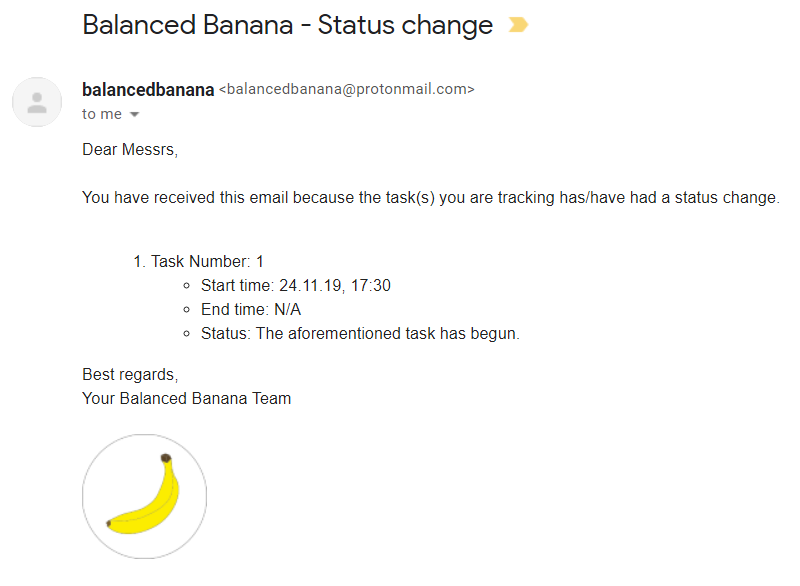
\includegraphics[width=\linewidth]{email_start.png}}
\end{center}

\clearpage
\subsubsection{Aufgabe beendet}
Dies ist ein Beispiel für eine E-Mail-Benachrichtigung, die ein Benutzer erhält, wenn eine Aufgabe abgeschlossen ist. Eine Aufgabe gilt als abgeschlossen, wenn sie erfolgreich ausgeführt wurde oder fehlgeschlagen ist. Die E-Mail-Benachrichtigung zeigt diesen Unterschied nicht an, es liegt an dem Benutzer, das Programm zu überprüfen, um zu sehen, ob die Aufgabe fehlgeschlagen ist oder nicht. Die Ausgabe des Programms wird in einer .txt-Datei gespeichert und in der E-Mail angehängt. \\

\begin{center}
	\makebox[\textwidth]{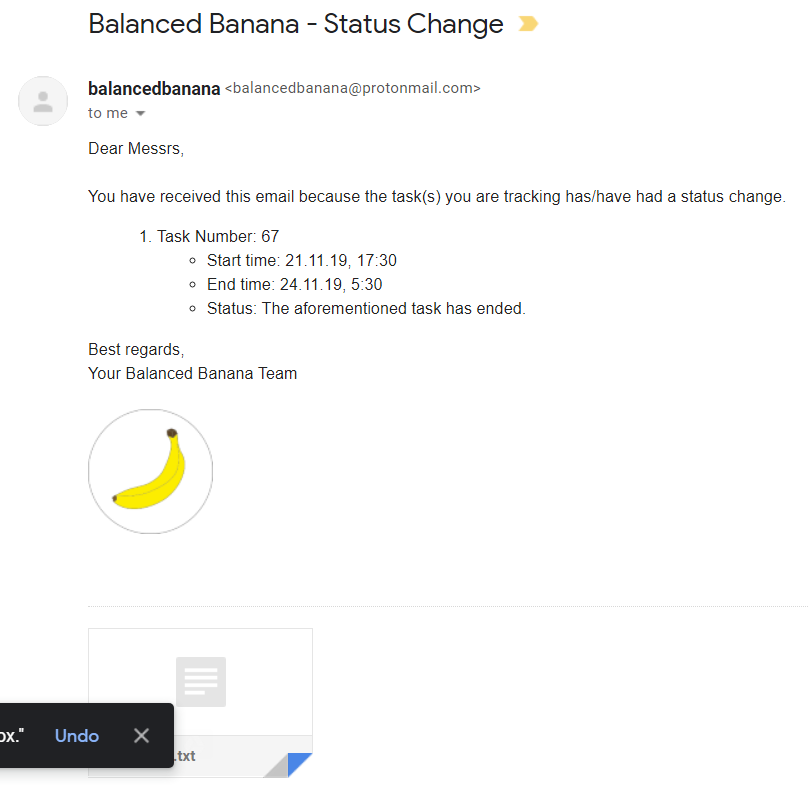
\includegraphics[width=\linewidth]{email_ended.png}}
\end{center}

\clearpage


\clearpage

\subsection{Befehlszeile}

\subsubsection{Hauptserver starten}
Startet das Programm im \gls{Daemon} Modus. Optional kann die Abhöhrende Internet Protokoll Adresse (v4 oder v6) und den Port (Dezimale 16bit Ganzzahl) im (lokalen) Netzwerk und der Http WebApi angeben werden.
\begin{mycode}
bbs [<--server|-s> <ipaddr>] [<--serverport|-sp> <port>] [<--webapi|-w> <ipaddr>] [<--webapi-port|-wp> <port>]
\end{mycode}

\subsubsection{Arbeiter starten}
Startet das Programm im \gls{Daemon} Modus. Optional kann die Internet Protokoll Adresse (v4 oder v6) bzw. der DNS Namen des Hauptservers und den Port (Dezimale 16bit Ganzzahl) im (lokalen) Netzwerk angeben werden.
\begin{mycode}
bbd [<--server|-s> <ipaddr>] [<--serverport|-sp> <port>]
\end{mycode}

\subsubsection{Aufgabe erstellen}
Sendet die angegebene Aufgabe an den Server und gibt die Aufgaben ID an der Standard Ausgabe aus (Dezimal).
\begin{mycode}
bbc <--run|-r> [--block|-b] [<--priority|-p> <priority>] [<--max-cpu-count|-Mc> <Integer>] [<--min-cpu-count|-mc> <Integer>] [<--max-ram|-Mr> <Integer>] [<--min-ram|-mr> <Integer>] [<--email|-em> <email>] [<--image|-im> <name>] [<program> [args]+]
\end{mycode}
Falls \texttt{-{}-block} block angegeben wurde, wird statt der Aufgaben ID die Ausgabe der Aufgabe ausgegeben.
Außer man beendet es forzeitig mit \texttt{CTRL + C}, dann wird die Aufgaben ID direkt danach ausgeben.

\subsubsection{Ausgabe der Aufgabe ansehen}
Gibt die gesammte Standardausgabe der angegebenen Aufgabe aus.
\begin{mycode}
bbc <--output|-o> <id>
\end{mycode}
\texttt{<id>} Aufgaben ID die beim erstellen der Aufgabe ausgegeben wurde.

\subsubsection{Ausgabe der Aufgabe ansehen}
Gibt nur die letzten Zeilen der Standardausgabe der angegebenen Aufgabe aus, bis man mit \texttt{CTRL + C} abbricht oder die Aufgabe sich beendet.
\begin{mycode}
bbc <--tail|-t> <id>
\end{mycode}
\texttt{<id>} Aufgaben ID die beim erstellen der Aufgabe ausgegeben wurde.

\subsubsection{Aufgaben sichern}
Erstellt einen Schnapschuss der Aufgabe, der später bei bedarf wiederhergestellt werden kann.
Gibt die Sicherungs ID an der Standard Ausgabe aus (Dezimal).
\begin{mycode}
bbc <--backup|-b> <id>
\end{mycode}
\texttt{<id>} Aufgaben ID die beim erstellen der Aufgabe ausgegeben wurde.

\subsubsection{Aufgaben fortsetzen}
Setzt die angehaltene Aufgabe fort.
\begin{mycode}
bbc <--continue|-c> <id>
\end{mycode}

\subsubsection{Aufgaben wiederherstellen}
\begin{mycode}
bbc <--restore|-r> <id> <backupid>
\end{mycode}
% \subsubsubsection{<backupid>} Zu viele ebenen
Sicherungs ID die beim erstellen der Sicherung ausgegeben wurde.

\subsubsection{Aufgaben pausieren}
Pausiert die Aufgabe mit der angegeben ID Nummer.
\begin{mycode}
bbc <--pause|-p> <id>
\end{mycode}

\subsubsection{Aufgaben beenden}
Beendet die Aufgabe mit der angegeben ID Nummer und git den exit Status der Aufgabe aus.
\begin{mycode}
bbc <--stop|-s> <id>
\end{mycode}

\subsubsection{Docker Abbild hinzufügen}
Fügt ein Docker Abbild als Ausführungsumgebung hinzu.
Legt sämtliche Eigenschaften eines Docker Abbildes mit einer \href{https://docs.docker.com/engine/reference/builder/}{DockerFile} fest.
Beispielsweise Betriebssystem und installierte Programme. 
\begin{mycode}
bbc <--add-image|-ai> <imagename> <Ordner der DockerFile>
\end{mycode}

\subsubsection{Docker Abbild entfernen}
Entfernt ein Docker Abbild als Ausführungsumgebung
\begin{mycode}
bbc <--remove-image|-ri> <imagename>
\end{mycode}

\subsubsection{\texttt{-{}-block}}
Kehrt erst nach der Ausführung der Aufgabe zum Aufrufer zurück. Nützlich um voneinander abhängige Aufgaben, in einem Konsolen Skript, nacheinander auszuführen.

\subsubsection{\texttt{-{}-priority}}
Legt die \gls{Prioritaet} der auszuführenden Aufgabe fest, gefolgt von low (4), medium (3), high (2), extreme (1), bananas (0).
Es kann der Name bzw. die Zahl in der Klammer als \gls{Prioritaet} verwendet werden.

\subsubsection{\texttt{-{}-min-cpu-count} und \texttt{-{}-max-cpu-count}}
Legen die minimale bzw. maximale anzahl der verwendbaren \glspl{CPU} fest.

\subsubsection{\texttt{-{}-min-ram} und \texttt{-{}-max-ram}}
Legen den minimal verfügbaren bzw. maximale verwendbaren Arbeitsspeicher fest.

\subsubsection{\texttt{-{}-server}}
Startet den Server, der die Aufgaben an die Arbeiter verteilt.


\clearpage
\section{Testfälle/Testszenarien}
\subsection{Grundlegende Testfälle}

\begin{itemize}
\item[T1] \textbf{Verbinden des Clients mit dem Server}
\subitem \textbf{Erklärung} Ziel ist zu testen, ob sich der Client beim Programstart automatisch mit dem Server verbinden kann.
\subitem \textbf{Ablauf} Ausgegangen wird von einem bereits laufenden System, das mindestens aus dem Server und einem Arbeiter besteht.
Der Nutzer versucht eine Aufgabe zu erstellen.
Wenn das System funktioniert, bekommt er die Job-Id seiner Aufgabe zurück.
Bekommt er die Fehlermeldung
\begin{mycode}
Error: Can not find server
\end{mycode}
so konnte keine Verbindung zum Server hergestellt werden. Erhält er die Fehlermelung
\begin{mycode}
Error: Could not authenticate to the server
\end{mycode}
so konnte der Nutzer sich nicht gegenüber dem Server authentisieren. Erhält er eine andere Fehlermeldung, so konnte die Aufgabe nicht gestartet werden.

\item[T2] \textbf{Festlegen von Prioritäten }
\subitem \textbf{Erklärung} Ziel ist zu testen, ob Aufgaben mit einer höheren \gls{Prioritaet} bevorzugt werden.
\subitem \textbf{Ablauf} Ausgegangen wird von einem bereits funktionierenden System mit genau einem Arbeiter, in dem Aufgaben verteilt und bearbeitet werden können.
Der Nutzer startet eine Aufgabe die einige Zeit benötigt. Während der Bearbeitung gibt er eine Aufgabe mit einer niedrigen \gls{Prioritaet} auf gefolgt von derselben Aufgabe mit einer hohen Priorität.
Sind alle drei Aufgaben bearbeitet, startet er wieder eine Aufgabe, die einige Zeit benötigt. Danach erstellt er eine Aufgabe mit einer hohen \gls{Prioritaet} und danach dieselbe Aufgabe mit niedriger Priorität.
Wenn das System korrekt funktioniert, werden in beiden Fällen die Aufgaben mit hoher \gls{Prioritaet} zuerst bearbeitet.

\item[T3] \textbf{Festlegen des Betriebssystems}
\subitem \textbf{Erklärung} Ziel ist zu testen, ob der Nutzer verschiedene Betriebssysteme angeben kann, die für die Bearbeitung seiner Aufgabe verwendet werden sollen.
\subitem \textbf{Ablauf} Ausgegangen wird von einem bereits funktionierenden System mit mehreren Arbeitern und mindestens zwei verschiedenen Arbeitern. Der Nutzer startet eine Aufgabe, die das Betriebssystem ausliest und ausgibt. Diese soll für jedes Betriebssystem einmal eingereiht werden mit einem Parameter, der das jeweilige Betriebssystem anfordert.

\item[T4] \textbf{Abfragen eines Aufgabenstatus }
\subitem \textbf{Erklärung} Ziel ist zu testen, ob der Nutzer den korrekten Status seiner Aufgaben abfragen kann.
\subitem \textbf{Ablauf} Ausgegangen wird von einem funktionierenden System mit genau einem Arbeiter, der Aufgaben entgegennehmen und verarbeiten kann.
Der Nutzer reiht mehrere Aufgaben mit unterschiedlichen Prioritäten ein. Die Aufgaben mit niedrigeren Prioritäten sollten in der Warteschlange sein und die Aufgaben mit höherer Priorität sollten entweder gestartet oder weiter vorne in der Warteschlange sein.

\item[T5] \textbf{Benachrichtigung bei Abschluss einer Aufgabe }
\subitem \textbf{Erklärung} Ziel ist zu testen, ob der Nutzer nach Abschluss einer Aufgabe vom System benachrichtigt wird.
\subitem \textbf{Ablauf} Ausgegangen wird von einem funktionierenden System, das in der Lage ist, Aufgaben anzunehmen und zu verarbeiten.
Der Nutzer reiht eine Aufgabe ein und prüft regelmäßig den Status seiner Aufgabe. Sollte die Aufgabe abgeschlossen sein, so sollte zeitnah eine Benachrichtigung per E-Mail folgen.

\item[T6] \textbf{Erstellen von Sicherungen}
\subitem \textbf{Erklärung} Ziel ist zu testen, ob das System regelmäßige Sicherungen seiner Aufgaben anlegt.
\subitem \textbf{Ablauf} Ausgegangen wird von einem funktionierenden System, das in der Lage ist, Aufgaben entgegenzunehmen und zu verarbeiten. Es wird eine Aufgabe eingereicht die hinreichend lange bearbeitet wird. Nach Ablauf eines Sicherungsintervalls wird im Dateisystem nach einer Sicherung der Aufgabe gesucht.

\item[T7] \textbf{Anforderung der Standard-Ausgabe }
\subitem \textbf{Erklärung} Ziel ist zu testen, ob der Nutzer in der Lage ist, sich die korrekte Standardausgabe seiner Aufgabe anzusehen
\subitem \textbf{Ablauf} Ausgegangen wird von einem funktionierenden System mit genau einem Arbeiter, das in der Lage ist, Aufgaben entgegenzunehmen und zu verarbeiten.
Der Nutzer reiht eine Aufgabe mit bekannter Ausgabe ein. Nach Abschluss der Aufgabe sollte die Ausgabe dieser entsprechen. Zusätzlich sollte der Abruf der Ausgabe einer nicht-existierenden Aufgabe eine Fehlermeldung ausgeben.
\end{itemize}

\subsection{Erweiterte Testfälle}

\begin{itemize}

\item[T8] \textbf{Abbrechen von zu langen Aufgaben }
\subitem \textbf{Erklärung} Ziel ist zu testen, ob der Server in der Lage ist, Aufgaben, die zu viel Zeit benötigen, abzubrechen.
\subitem \textbf{Ablauf} Ausgegangen wird von einem funktionierenden System, das in der Lage ist Aufgaben entgegenzunehmen und zu verarbeiten und den Auftraggeber nach Abschluss einer Aufgabe zu benachrichtigen.
Der Nutzer reiht eine Aufgabe ein, die nicht beendet. Nach einem festen Zeitintervall sollte der Benutzer eine Benachrichtigung über den erzwungenen Abschluss seiner Aufgabe erhalten.

\item[T9] \textbf{Manuelles Stoppen von Aufgaben }
\subitem \textbf{Erklärung} Ziel ist zu testen, ob der Nutzer in der Lage ist, seine Aufgaben selbst abzubrechen.
\subitem \textbf{Ablauf} Ausgegangen wird von einem funktionierenden System, das in der Lage ist Aufgaben entgegenzunehmen, zu verarbeiten und den Status von Aufgaben zurückzugeben.
Der Nutzer reiht eine Aufgabe ein und fordert im Anschluss den Stopp der Aufgabe. Bei einer Statusabfrage sollte die Aufgabe nun als gestoppt angezeigt werden.

\item[T10] \textbf{Manuelle Sicherung von Aufgaben}
\subitem \textbf{Erklärung} Ziel ist zu testen, ob der Nutzer seine Aufgaben manuell sichern kann.
\subitem \textbf{Ablauf} Ausgegangen wird von einem System, das in der Lage ist, Aufgaben entgegenzunehmen und zu bearbeiten.
Der Nutzer reiht eine Aufgabe ein und fordert im Anschluss daran die manuelle Sicherung dieser. Im Dateisystem wird nach der Sicherung dieser Aufgabe gesucht.

\end{itemize}

\clearpage
\printnoidxglossaries

\end{document}
